\documentclass[letterpaper]{article}

\usepackage{amsmath}
\usepackage{amssymb}
\usepackage{amsthm}
\usepackage{commath}
\usepackage{enumerate}
\usepackage{lmodern}
\usepackage{microtype}
\usepackage{fullpage}
\usepackage{graphicx}
\usepackage[cache=false]{minted}
\usepackage{hyperref}

\title{STAT 527: Assignment \#4}
\author{Philip Pham}
\date{\today}

\DeclareMathOperator{\E}{E}
\DeclareMathOperator{\Prob}{P}

\begin{document}
\maketitle

\section*{Problem 1}

\begin{figure}[h!]
  \centering
  \caption{Plots of $n^{-1}\sum_{i=1}^n \left(f(x) - \hat{f}(x)\right)^2$, where
    $n = 128$ and $128$ simulations were run.}
  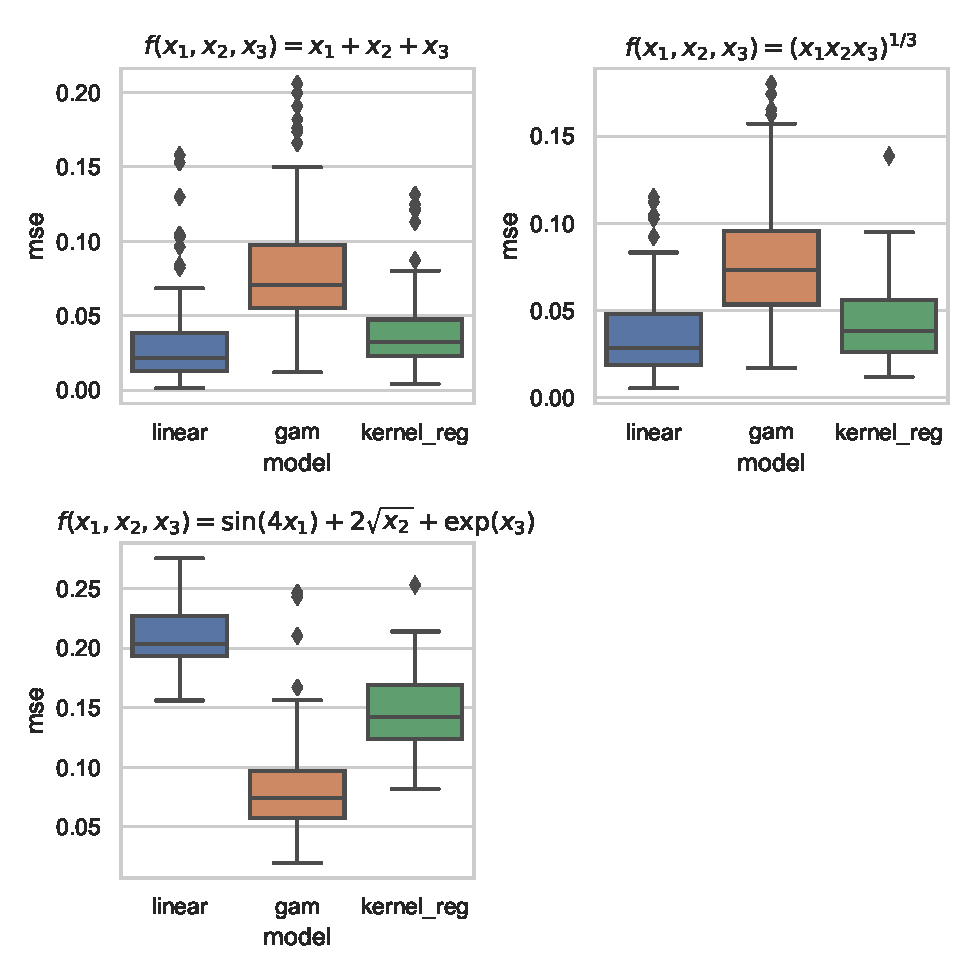
\includegraphics[width=0.75\textwidth]{mse.pdf}
\end{figure}

I ran simulations with the various models.
\begin{description}
\item[\texttt{linear}:] A multivariate linear regression.
\item[\texttt{gam}:] A generalized additive model with cubic splines. Degrees of
  freedom was of 4 was chosen with a simple sweep over all possible values.
\item[\texttt{kernel\_reg}:] A linear local regression with Gaussian kernel. A
  bandwidth of $0.5$ was chosen with a simple sweep over the interval
  $[0.01, 1]$.  
\end{description}

When the data is linear, unsurprisingly the linear model does best. This is
the true model, so we would expect no bias and the minimal possible
variance. Local linear regression also does well here, for the relationship is
also locally linear, but the variance is higher. The generalized additive
model does poorly. Since it is a generalization of the linear regression, it
is unbiased, but it overfits to the noise, so the variance is greater.

When $f(x_1, x_2, x_3) = \sin(4x_1) + 2\sqrt{x_2} + \exp(x_3)$, the linear
model does very poorly as it is very biased. The generalized additive model
does the best with these nonlinearities, while the local linear regression is
compromise between the two.

When $f$ is the geometric mean, $f$ is close enough to linear, that the linear
model and local linear regression do better.

In higher dimensions, the local linear regression, would likely fare poorly
since it depends on nearest neighbor calculations, so the variance would becomes
large. The more structured generalized additive models and especially
linear regression should do better here despite their bias.
\section*{Problem 2}

I'll try and work on my final project.

\end{document}
%%% Local Variables:
%%% TeX-command-extra-options: "-shell-escape"
%%% End: